

\section{Estudio de Factibilidad}

Como se expuso anteriormente, el protocolo criptográfico nos arroja excelentes beneficios en cuanto a la optimización de espacio de memoria en la nube y garantiza la seguridad e integridad de los datos de usuarios registrados en la nube. Hasta ahora se tiene muy claro cuál será el impacto de la implementación de este protocolo, pero aún queda por establecer cuán viable es la realización de este protocolo en cuanto a facilidades técnicas y operativas.


\subsection{Factibilidad técnica}

Para la implementación del protocolo criptográfico, se cuentan con las herramientas de software necesarias ya que estas existen y están disponibles para su uso y disponibilidad inmediata al desarrollo del protocolo. Cabe mencionar que las herramientas que involucran todo el desarrollo del protocolo, se encuentran completas en tanto a funcionalidades, soportes, documentación, seguridad, etc. 
En cuanto a los conocimientos necesarios al protocolo, se cuentan con los suficientes que este protocolo necesita para su applicación. Dichos conocimientos se han adquirido a lo largo de la estadía en la ingeniería mediante las clases recibidas en las instalaciones de la  escuela o por la adquisición por medios externos. Ahora bien, un pequeño inconveniente para la aplicación del protocolo, es el desarrollo del software, ya que existen partes fundamentales del protocolo que requieren de nuevo conocimiento que aun no se adquiere y es necesario aprender, por tanto existe una pequeña posibilidad de que esto signifique un retraso en la producción del protocolo. 

\begin{itemize}

	\item \textbf{Lenguaje de programación:} para el desarrollo del sistema se estará trabajando con varios lenguajes de programación, la base de este desarrollo será Python, ya que es un lenguaje de fácil comprensión y con una lógica bastate familiar a lenguajes que anteriormente se habían trabajado, además de que Python nos permite trabajar primitivas criptográficas con una mayor facilidad. \\
	\item \textbf{Sistema gestor de base de datos:} Se implementará MySQL como un manejador de base de datos, ya que es software libre y además se cuenta con una mayor experiencia de manejo y entendimiento. 
\\
De acuerdo con los requerimientos del sistema, los componentes necesarios para la implementación de este protocolo son: 

	\item \textbf{Hardware} 
Se requiere de equipo de cómputo para poder llevar a cabo la codificación del protocolo y la configuración de los servidores que le darán soporte a las actividades realizadas en la interacción del usuario con el sistema. El equipo de trabajo cuenta con 3 computadoras personales (LAPTOP) que son las siguientes: 
\begin{longtable}{ |  p{5cm} |  p{10.5cm} |}

% aquí añadimos el encabezado de la primera hoja.
\hline
\multicolumn{2}{|c|}{\textbf{Componentes Físicos (Hardware)}} \\ \hline
\textbf{Componente} & \textbf{Características} \\
\hline \hline
\endfirsthead

% aquí añadimos el encabezado del resto de hojas.
\hline
\textbf{Componente} & \textbf{Características} \\
\hline \hline
\endhead

% aquí añadimos el fondo de todas las hojas, excepto de la última.
\multicolumn{2}{|c|}{Continua en la siguiente página.}
\endfoot

% aquí añadimos el fondo de la última hoja.
\endlastfoot

Laptop HP Pavilion g4 & \begin{itemize}
				\item Procesador: AMD A6-4400M APU 2.70Hz
				\item Memoria RAM: 8.00GB 
				\item Disco Duro: 750GB
				\item Tipo Sistema: 64bits x64
			      \end{itemize} \\ \hline

Laptop Acer Aspire V5 &  \begin{itemize}
				\item Procesador: Intel(R) Celeron(R)  1.50GHz 
				\item Memoria RAM: 2.00GB
				\item Disco Duro: 250GB
				\item Tipo Sistema: 64bits x64
			      \end{itemize} \\ \hline

Laptop HP probook &  \begin{itemize}
				\item Procesador: AMD Phenom(tm) ll X2 545  3.00GHz 
				\item Memoria RAM: 4.00GB
				\item Disco Duro: 350GB
				\item Tipo Sistema: 64bits x64
			      \end{itemize} \\ \hline

Servidor ownCloud &  \begin{itemize}
				\item Servicio de alojamiento de archivos con almacenamiento en la nube
				\item Servidores de instalación: PHP, SQLite. MySQL, PostgreSQL
				\item Servidor de archivos: WebDAV
				\item Calendario de sincronzación: CardDAV
				\item Sistema operativo: MMultiplataforma
			      \end{itemize} \\ \hline
\caption{Componentes físicos}
\label{Hardware}
\end{longtable}

	\item \textbf{Software}
Con respecto al software, no se pretende usar un sistema operativo en específico ya que el servicio de la nube es compatible con cualquier sistema operativo en que se esté desarrollando. Sin embargo se cuenta con los siguientes sitemas operativos: 

\begin{table}[htb]
\centering
\begin{tabular}{| p{5cm} |  p{10.5cm} |}
\hline
\multicolumn{2}{|c|}{\textbf{Softawe}} \\ \hline
\textbf{Tipo} &  \textbf{Cantidad} \\
\hline \hline
S.O. Windows 8.1 Pro & 2\\ \hline
S.O. Windows 10 Pro & 1\\ \hline

\end{tabular}
\caption{Componentes Lógicos}
\label{Servidor de Llaves }
\end{table}
\end{itemize}



\subsection{Factibilidad operativa}
El uso e implantación de este protocolo criptográfico, tiene como principal objetivo el eliminar las duplicaciones de archivos que se almacenan en la nube y de igual manera el evitar los ataques de adversarios por fuerza bruta a la información de los ususrios en la nube , por lo cual resulta factible la operación del proyecto, ya que se esta proponiendo una solución de bajo costo con grandes eneficios.
Hoy en día va en aumento el número de usuarios de la nube, ya sean empresas, organizaciones, personas, etc. todos estos usuarios buscan su información rapido y de fácil acceso en cualquier lugar con una conexión a internet, y esto hace que también caumente la cantidad de información almacenada que en ocasiones está replicada en uno o mas usuarios.
Este protocolo pretende atender al problema del crecimiento en la infraestructura de la nube ofreciendo una solución para contrarestarlo y de esa manera más usuarios podrán tener acceso a la nube sin necesidad de aumentar a la infraestructura de esta.

\subsection{Facctibilidad económica}
El estudio de factibilidad económica nos permite analizar los costo - beneficios monetarios que se obtendrán con el desarrollo del proyecto, ya que dicho protocolo en un largo plazo podría comenzar en producción industrial para su comercialización y districución en el mercado de las tecnologías de la información, ya que proveerá de servicios en el cómputo nube que hoy en día las empresas están optando por invertir en el y optimizar sus recursos y procesos del negocio. 

En cuanto al análisis de el gasto económico que se requiere para la implementación y la realización de pruebas del protocolo, existe un beneficio ya que todos los componentes para el desarrollo del sistema son libres,es decir que no se realizará la adquisición de licencias de desarrollo ni programas para la implementación. 
\\ El servidor que nos proveerá del almacenamiento en la nube de nombre \textbf{ownCloud.org} es de libre acceso y no existe restricción alguna para la utilización de este. Nos permite una libre manipulación y configuración de tal modo que podamos cumplir nuestros objetivos.


\subsection{Análisis de riesgos} 

EL análisis de riesgos consiste en identificar los riesgos que este sistema puede tener en su futura implementación y desarrollo. Este análisis presenta los riesgos identificados en el sistema y 3 indicadores (Prioridad, Probabilidad e Impacto) fundamentales para llevar a cabo la gestión de riesgos y así tener presente cuales son los riesgos más destacados en el sistema para dimensionar las consecuencias que estos podrían traer consigo si llegaran a ocurrir. Para elaborar este análisis de riesgos, se evaluaron los impactos que estos riesgos pueden traer, mediante 5 escalas de impactode un riesgo, dichas escalas son: 

\subsubsection{Escalas de impacto de un riesgo}
\begin{longtable}{| p{2.5cm} |  p{2.5cm} |  p{2.5cm} |  p{2.5cm} |  p{2.5cm} |  p{2.7cm} |}

% aquí añadimos el encabezado de la primera hoja.
\hline
\multicolumn{6}{|c|}{\textbf{Escalas de impacto de un riesgo}} \\ \hline
\textit{\textbf{Objetivo del proyecto}} &  \textbf{Muy bajo/ 0.05} & \textbf{Bajo/ 0.10} & \textbf{Moderado/ 0.20} & \textbf{Alto/ 0.40} & \textbf{Muy alto/ 0.80}\\
\hline \hline
\endfirsthead

% aquí añadimos el encabezado del resto de hojas.
\hline
\textit{\textbf{Objetivo del proyecto}} &  \textbf{Muy bajo/ 0.05} & \textbf{Bajo/ 0.10} & \textbf{Moderado/ 0.20} & \textbf{Alto/ 0.40} & \textbf{Muy alto/ 0.80}\\
\hline \hline
\endhead

% aquí añadimos el fondo de todas las hojas, excepto de la última.
\multicolumn{6}{|c|}{Continua en la siguiente página}
\endfoot

% aquí añadimos el fondo de la última hoja.
\endlastfoot


\textbf{Costo} & Aumento insignificante de costo & Aumento del costo <10\% &  Aumento del costo 10 - 20\% & Aumento del costo 20 - 40\% & Aumento del costo >40\%  \\ \hline
\textbf{Tiempo} & Aumento insignificante de tiempo & Aumento del tiempo <5\% &  Aumento del tiempo 5 - 10\% & Aumento del tiempo 10 - 20\% & Aumento del tiempo >20\%  \\ \hline
\textbf{Alcance} & Disminución del alcance apenas perceptible & Áreas de alcance secundarias afectadas & Áreas de alcance principales afectadas & Reducción del alcance inaceptable para los objetivos &  El producto terminado es inservible\\ \hline
\textbf{Calidad} & Degradación de calidad apenas perceptible & Sólo las aplicaciones muy exigentes se ven afectadas & La reducción de la calidad requiere aprobación externa & Reducción de calidad inaceptable &  El producto terminado es inservible\\ \hline


\caption{Escalas de impacto de un riesgo}
\label{Riesgos}
\end{longtable}

\begin{longtable}{| p{1cm} | p{4cm} | p{2cm} | p{2.5cm} | p{2cm} | p{4cm} |}

% aquí añadimos el encabezado de la primera hoja.
\hline
\multicolumn{6}{|c|}{\textbf{Análisis de riesgos}} \\ \hline
\textbf{ID} &  \textbf{Riesgo} & \textbf{Prioridad} & \textbf{Probabilidad} & \textbf{Impacto} & \textbf{Causa}\\
\hline \hline
\endfirsthead

% aquí añadimos el encabezado del resto de hojas.
\hline
\textbf{ID} &  \textbf{Riesgo} & \textbf{Prioridad} & \textbf{Probabilidad} & \textbf{Impacto} & \textbf{Causa}\\
\hline \hline
\endhead

% aquí añadimos el fondo de todas las hojas, excepto de la última.
\multicolumn{6}{|c|}{Continua en la siguiente página.}
\endfoot

% aquí añadimos el fondo de la última hoja.
\endlastfoot

% aquí añadimos el cuerpo de la tabla.
R1 & Modificar requerimientos &  ALTA & MEDIA & ALTO & Nuevas características del protocolo \\ \hline
R2 & Cambios en tecnología & BAJA & MEDIA & BAJO & La tecnología usada es menos eficiente y causa conflictos \\ \hline
R3 & Falta de usuarios y peticiones & ALTA & BAJA &  BAJO & No se localizaron todos los involucrados en el protocolo \\ \hline
R4 & Equipo de cómputo & ALTA & BAJA & MUY BAJO & El equipo de cómputo empleado falla o no se encuentra funcionando \\ \hline
R5 & Incumplimiento de acuerdos & ALTA & ALTA & MODERADO & Retrazo en actividades prgramadas \\ \hline
R6 & Problemas de planeación & MEDIA & ALTA & ALTO & Falta de comunicación por parte del equipo \\ \hline
R7 & Falta de recursos & ALTA & MEDIA & MUY ALTO & No se cuenta con el poder adquisitivo de recursos e insumos \\ \hline
R8 & Falta de conocimientos & MEDIA & MEDIA & MUY ALTO & El equipo no se encuentra capacitado para el desarrollo del sistema. \\ \hline
R9 & Sobre estimación de insumos & MEDIA & MEDIA & MODERADO & Los insumos para la implementación del sistema no son los adeacuados para el desarrollo. 

\\ \hline
\caption{Análisis de riesgos del proyecto}
\label{Análisis de riesgos }
\end{longtable}

%=============================================================================================================================================================


\section{Arquitectura del sistema. }

\begin{figure}[H]
\centering
	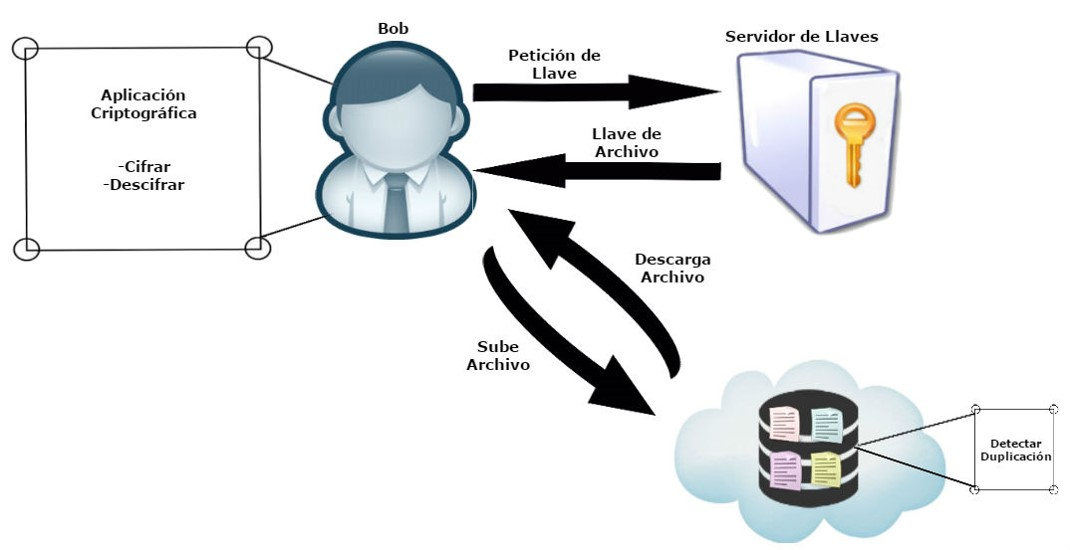
\includegraphics[width=16cm, height=11cm]{./images/Arqui.jpg}
	\caption{Arquitectura general del sistema.}

\end{figure}

%\begin{figure}[H]
%\centering
%	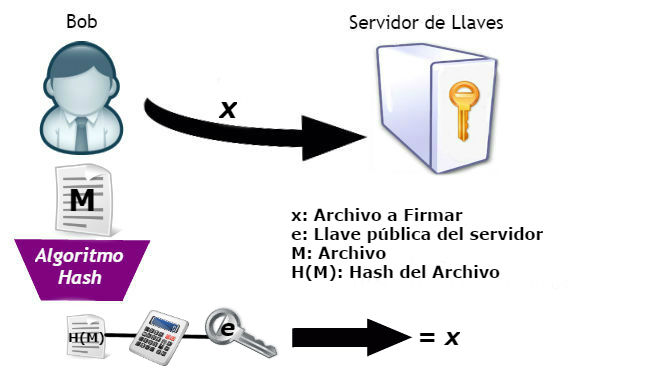
\includegraphics[width=16cm, height=11cm]{./images/Paso01.jpg}
%	\caption{Arquitectura del sistema paso 1.}

%\end{figure}

%\begin{figure}[H]
%\centering
%	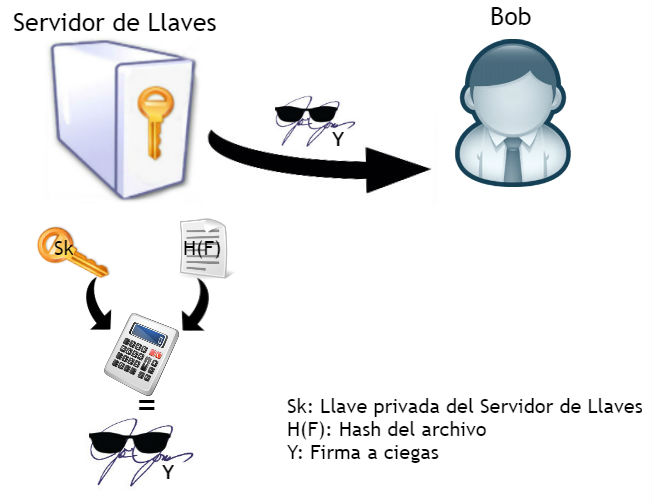
\includegraphics[width=16cm, height=13cm]{./images/Paso02.jpg}
%	\caption{Arquitectura del sistema paso 2.}

%\end{figure}

%\begin{figure}[H]
%\centering
%	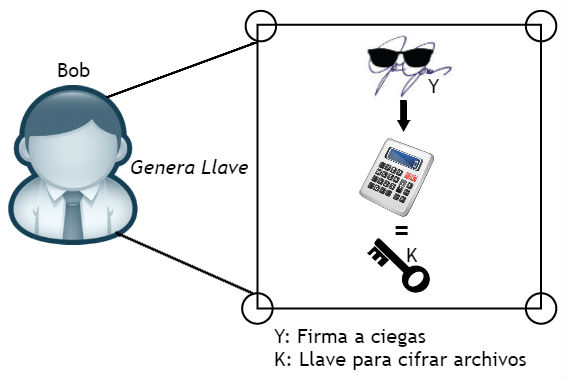
\includegraphics[width=16cm, height=10cm]{./images/Paso03.jpg}
%	\caption{Arquitectura del sistema paso 3.}

%\end{figure}

%\begin{figure}[H]
%\centering
%	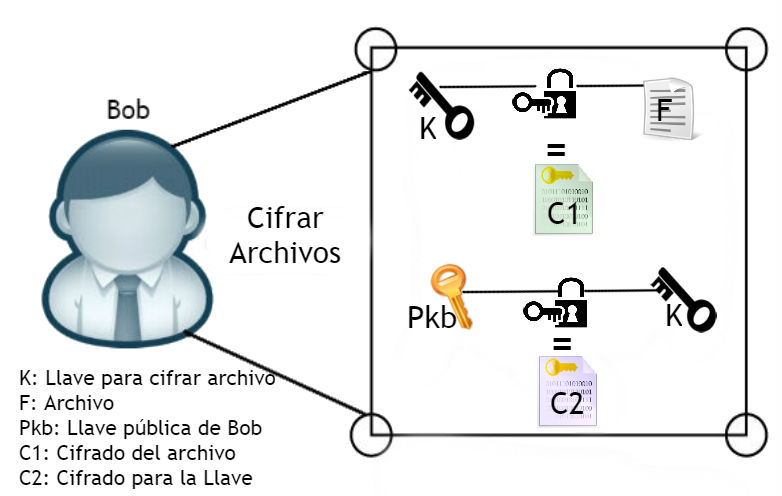
\includegraphics[width=16cm, height=10cm]{./images/Paso04.jpg}
%	\caption{Arquitectura del sistema paso 4.}

%\end{figure}

%=============================================================================================================================================================
\section{Descripcion de procesos}

\subsection{Descripción del proceso subir archivo.}

El proceso inicia cuando el cliente desea subir un archivo nuevo, el cliente debe dar clic en la opción de subir archivo y seleccionar el archivo que desee subir, el sistema va a calcular el hash del archivo elegido, después hará unas operaciones aritméticas con el has para generar una x que se enviara al servidor para que realice una firma a ciegas, y con esta firma que se le regresara al cliente, se va a generar del lado del cliente su llave "k" que será la llave con la cual cifrara el archivo, y así si otro archivo que se quiera subir es igual a este tendrá la misma k y podrá el sistema detectar que son duplicados, también el sistema va a cifrar la llave k por si se le llega a perder al cliente, para poder almacenarlo en la nube el sistema mandara el hash del archivo cifrado para ver si ya está registrado en la base de datos, si es así solo guarda la llave y actualiza la lista de los usuario que comparten el archivo, de lo contrario solicita la llave cifrada y el archivo cifrado para almacenarlos y actualiza su lista de usuario añadiendo un archivo en ella, y por último se le notificará al cliente que su archivo ha sido almacenado.



% - - - - - - - - - - - - - - - - - - - - - - - - -
\subsubsection{Participantes}

\begin{tabular}{ |p{2cm}|p{6cm}|p{6cm}|  }
\hline
\multicolumn{3}{|c|}{  Participantes  } \\
\hline

{ Nombre }  & { Descripción } & { Responsabilidades} \\
\hline
{ Servidor } &  Actor que realiza la firma a ciegas del archivo.  &  
			\begin{itemize}	
				\item Frima a ciegas.

			\end{itemize}   \\ 
\hline
{ Cliente } &   Actor que sube archivos a la Nube.  &  
			\begin{itemize}	
				\item Selecciona archivo a subir.
				\item Genera hash del archivo. 
				\item Calcula la llave k.
				\item Cifra los archivos a subir.
			\end{itemize}   \\ 
\hline
{ Nube } &   Actor que almacena los archivos.  &  
			\begin{itemize}	
				\item Almacena los archivos seleccionados.
				\item Genera lista de usuarios relacionados.
			\end{itemize}   \\ 
\hline
\end{tabular}


\begin{figure}[H]
\centering
	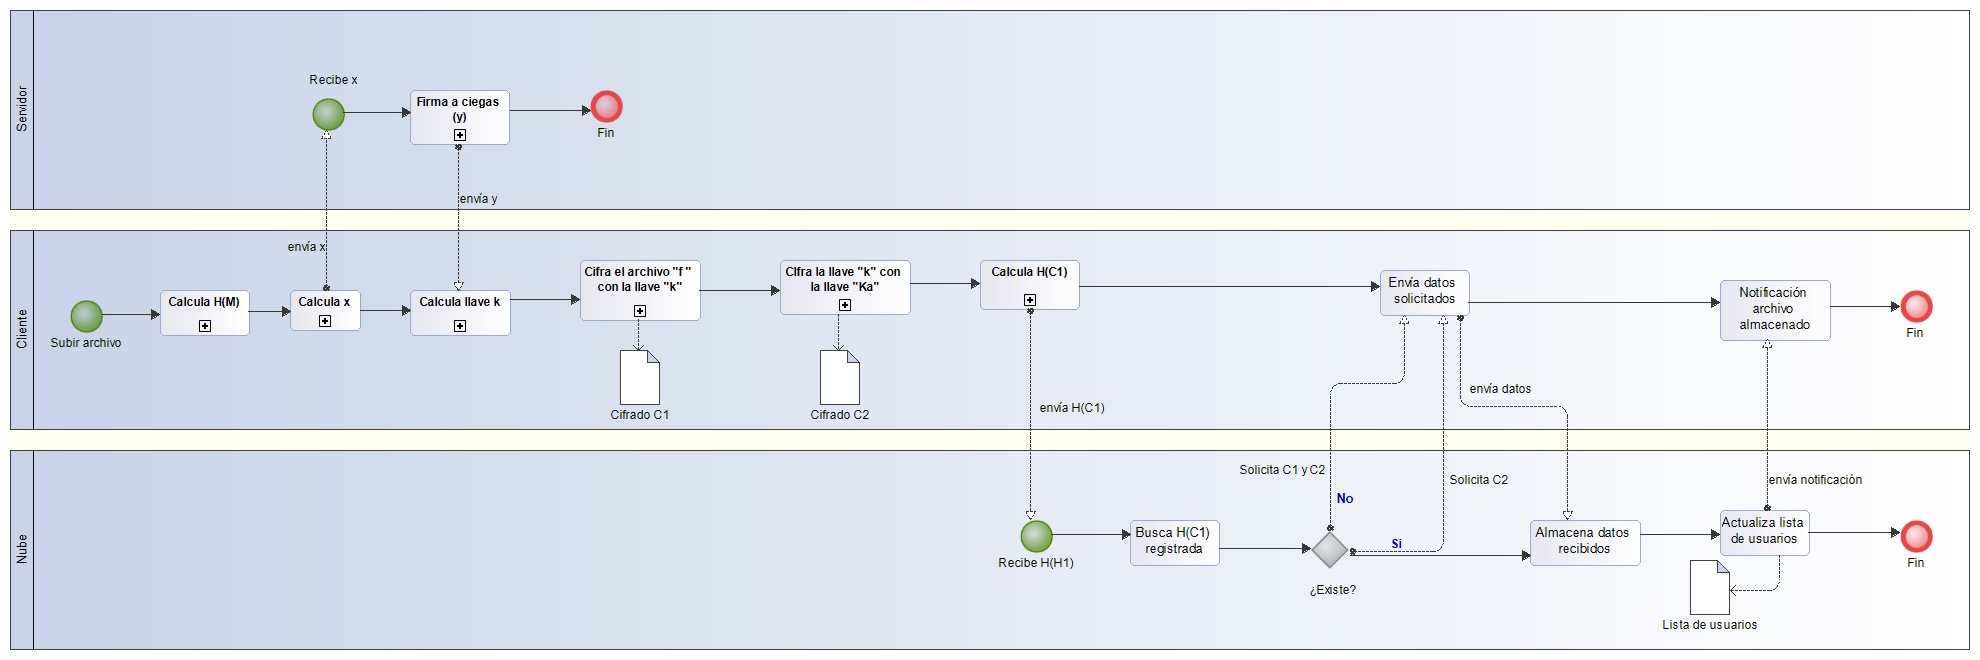
\includegraphics[width=16cm, height=7cm]{./images/BPM_Subir.png}
	\caption{BPMN Subir archivo.}

\end{figure}


\subsection{Descripción del proceso Descargar archivo.}

El proceso inicia cuando el cliente desea descargar un archivo, el cliente debe dar clic en la opción de descargar archivo y seleccionar el archivo que desee descargar, el sistema va a mandar el nombre del archivo a la nube para que busque en su base de datos los archivos correspondientes al usuario y nombre del archivo, se le regresaran al cliente y el sistema en el lado del cliente deberá descifrar el archivo C2 que contiene la llave k para poder descifrar el otro archivo C1 donde se encuentra el archivo original, el sistema notificara al cliente que su archivo se ha descargado con éxito y este podrá abrirlo. \\


% - - - - - - - - - - - - - - - - - - - - - - - - -
\subsubsection{Participantes}

\begin{tabular}{ |p{2cm}|p{6cm}|p{6cm}|  }
\hline
\multicolumn{3}{|c|}{  Participantes  } \\
\hline

{ Nombre }  & { Descripción } & { Responsabilidades} \\
\hline
{ Cliente } &   Actor que descarga archivos de la Nube.  &  
			\begin{itemize}	
				\item Selecciona archivo a descargar.
				\item Descifra los archivos descargados.
			\end{itemize}   \\ 
\hline
{ Nube } &   Actor que almacena los archivos.  &  
			\begin{itemize}	
				\item Almacena los archivos seleccionados.
				\item Genera lista de usuarios relacionados.
				\item Enviar los archivos a descargar.
			\end{itemize}   \\ 
\hline
\end{tabular}

\begin{figure}[H]
\centering
	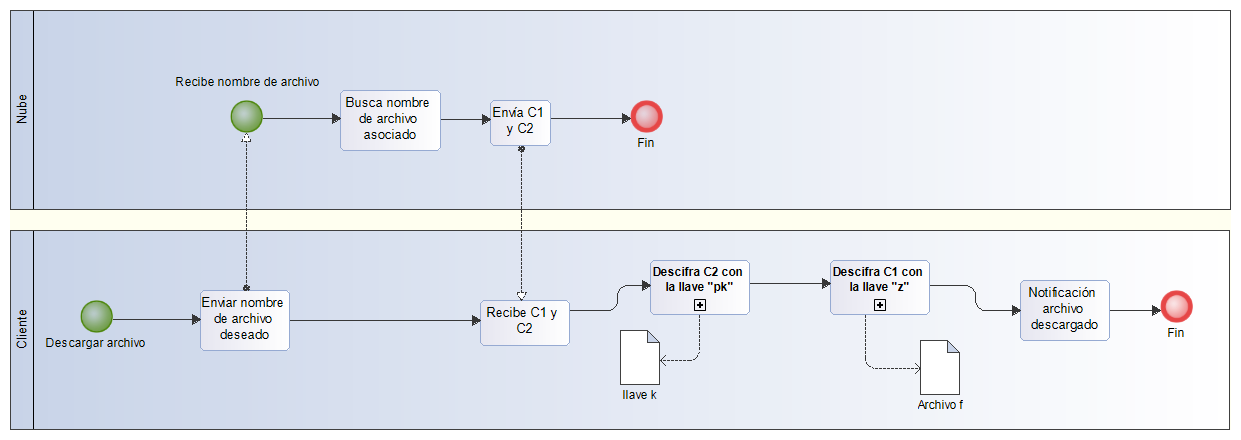
\includegraphics[width=16cm, height=7cm]{./images/BPM_Descargar.png}
	\caption{BPMN Descargar archivo.}

\end{figure}

\vspace{3cm}
\subsection{Descripción del proceso eliminar archivo.}

El proceso inicia cuando el cliente desea eliminar un archivo nuevo, el cliente debe dar clic en la opción de eliminar archivo y seleccionar el archivo que desee eliminar, el sistema va a enviar el nombre del archivo a la nube donde este buscara en su base de datos los archivos que corresponden al usuario y nombre del archivo, los va a eliminar de su base de datos y actualizara su lista de usuarios eliminado de ella los datos del archivo y usuario que coinciden con el archivo eliminado, se le enviara una notificación al cliente que su archivo ha sido eliminado con éxito de la nube.\\



% - - - - - - - - - - - - - - - - - - - - - - - - -
\subsubsection{Participantes}

\begin{tabular}{ |p{2cm}|p{6cm}|p{6cm}|  }
\hline
\multicolumn{3}{|c|}{  Participantes  } \\
\hline

{ Nombre }  & { Descripción } & { Responsabilidades} \\
\hline
{ Cliente } &   Actor que elimina archivos de la Nube.  &  
			\begin{itemize}	
				\item Selecciona archivo a elminar.
			\end{itemize}   \\ 
\hline
{ Nube } &   Actor que almacena los archivos.  &  
			\begin{itemize}	
				\item Elimina los archivos seleccionados.
				\item Genera lista de usuarios relacionados.
			\end{itemize}   \\ 
\hline
\end{tabular}

\begin{figure}[H]
\centering
	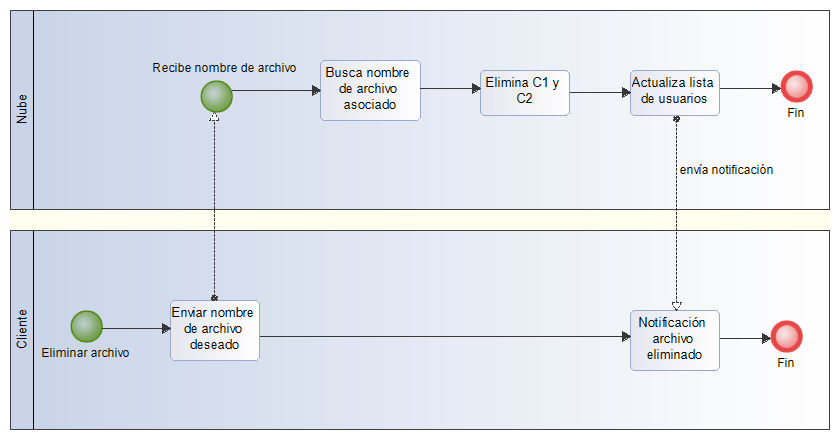
\includegraphics[width=16cm, height=7cm]{./images/BPM_Eliminar.png}
	\caption{BPMN Eliminar archivo.}

\end{figure} 

\newpage
%=======================================================================================================================================
\section{Modelo de entidades. }

\subsection{Diagrama de Entidad Relación. }

\begin{figure}[H]
\centering
	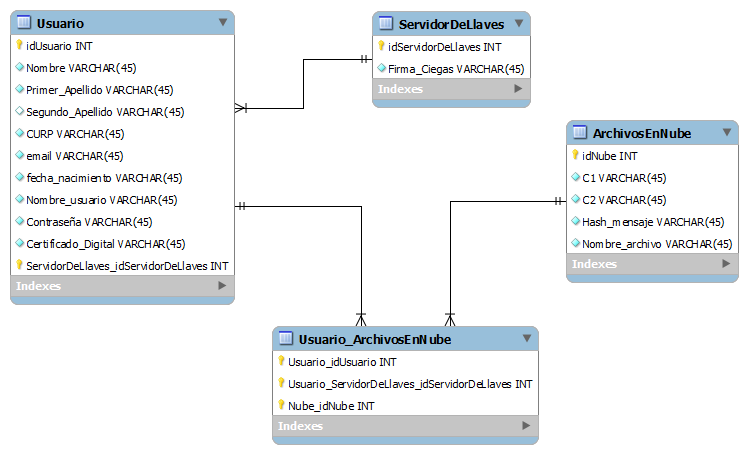
\includegraphics[width=16cm, height=10cm]{./images/BDTT2.png}
	\caption{Diagrama Entidad relación del sistema.}

\end{figure} 

\newpage

\subsection{Diagrama de clases. }

\begin{figure}[H]
\centering
	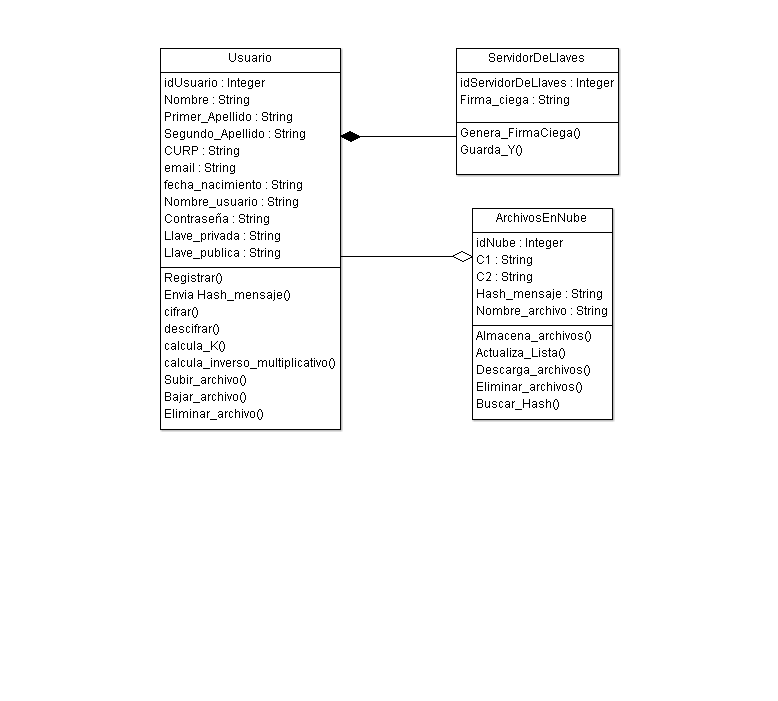
\includegraphics[width=18cm, height=15cm]{./images/DiagramaClasesTT.png}
	\caption{Diagarama de clases del sistema.}

\end{figure} 
\newpage
%=======================================================================================================================================
\section{Requerimientos Funcionales. }

\begin{table}[htb]
\centering
\begin{tabular}{| p{2cm} |  p{13.5cm} |}
\hline
\multicolumn{2}{|c|}{\textbf{Requerimientos funcionales del protocolo}} \\ \hline
\textbf{ID} &  \textbf{Descripción} \\
\hline \hline
RF1 & El sistema permitirá el registro de un nuevo usuario \\ \hline
RF2 & El sistema permitirá al usuario iniciar sesión para comenzar a manipular su información \\ \hline
RF3 & El sistema permitirá al usuario gestionar su perfil para la visualización, actualización y configuración de su información \\ \hline
RF4 & El sistema permitirá al usuario gestionar los archivos que dicho usuario tiene registrado en su perfil \\ \hline

\end{tabular}
\caption{Requerimientos funcionales del servidor de llaves}
\label{Servidor de Llaves }
\end{table}




\begin{table}[htb]
\centering
\begin{tabular}{| p{2cm} |  p{13.5cm} |}
\hline
\multicolumn{2}{|c|}{\textbf{Servidor de Llaves}} \\ \hline
\textbf{ID} &  \textbf{Descripción} \\
\hline \hline
RF – SLL1 &El sistema permitirá la generación de llaves de usuario a través de las llaves pública y privada  del servidor de llaves \\ \hline
RF – SLL2 & El sistema permitirá la firma a ciegas (y) de cualquier archivo que se desee almacenar\\ \hline
\end{tabular}
\caption{Requerimientos funcionales del servidor de llaves}
\label{Servidor de Llaves }
\end{table}


\begin{table}[htb]
\centering
\begin{tabular}{| p{2cm} |  p{13.5cm} |}
\hline
\multicolumn{2}{|c|}{\textbf{Cliente}} \\ \hline
\textbf{ID} &  \textbf{Descripción} \\
\hline \hline
RF – CL1 & El sistema permitirá al usuario gestionar archivos: Subir, Descargar, Eliminar \\ \hline
RF – CL2 & El sistema permitirá al usuario subir un archivo (F) cifrado al servicio de almacenamiento   \\ \hline
RF – CL3 & El sistema permitirá al usuario descargar un archivo (F) descifrado elejido de su lista de archivos en el servicio de almacenamiento. \\ \hline
RF – CL4 &El sistema permitirá al usuario eliminar un archivo (F) cuando el usuario elige alguno de su lista de archivos cargados en el servicio de almacenamiento.   \\ \hline
\end{tabular}
\caption{Requerimientos funcionales del cliente}
\label{Cliente }
\end{table}


\begin{table}[htb]
\centering
\begin{tabular}{| p{2cm} |  p{13.5cm} |}
\hline
\multicolumn{2}{|c|}{\textbf{Servicio de almacenamiento (Nube)}} \\ \hline
\textbf{ID} &  \textbf{Descripción} \\
\hline \hline

RF – N1 & El sistema permitirá al servicio de almacenamiento llevar a cabo un proceso para la detección de archivos duplicados.  \\ \hline

\end{tabular}
\caption{Requerimientos funcionales del Servicio de almacenamiento (Nube)}
\label{Servicio de almacenamiento (Nube) }
\end{table}
%=======================================================================================================================================
\vspace{9cm}
\section{Requerimientos No Funcionales }
\begin{longtable}{| p{1.5cm} | p{3cm} | p{11cm} |}

% aquí añadimos el encabezado de la primera hoja.
\hline
\multicolumn{3}{|c|}{\textbf{Requerimientos No Funcionales}} \\ \hline
\textbf{ID} &  \textbf{Atributo} & \textbf{Descripción}\\
\hline \hline
\endfirsthead

% aquí añadimos el encabezado del resto de hojas.
\hline
\textbf{ID} &  \textbf{Atributo} & \textbf{Descripción}\\
\hline \hline
\endhead

% aquí añadimos el fondo de todas las hojas, excepto de la última.
\multicolumn{3}{|c|}{Continua en la siguiente página}
\endfoot

% aquí añadimos el fondo de la última hoja.
\endlastfoot

% aquí añadimos el cuerpo de la tabla.
RNF1 & Eficiencia &  \begin{itemize} 
   \item El servidor de llaves tendrá la capacidad de realizar 1000 peticiones de gestión de almacenamiento de archivos por segundo. 
   \item El sistema podrá funcionar de forma correcta con usuarios conectados de manera concurrente. 
   \item Los archivos que sean gestionados dentro del servidor de almacenamiento, deben ser actualizados en la base datos y la visualización de cada cliente de manera casi inmediata. 
  \end{itemize}
\\ \hline

RNF2 & Fiabilidad &  \begin{itemize} 
  \item La pérdida de consultas en el servidor de llaves es menor a 3 veces el máximo de consultas realizadas. 
   \item Los archivos almacenados en el servidor de almacenamiento deben ser recuperados por el usuario al instante en que este lo solicite. 
   \item El tiempo de latencia que existe entre el servidor de llaves y el cleinte será de máximo 118ms. 
 \end{itemize}
\\ \hline

RNF3 & Seguridad & \begin{itemize} 
    \item El sistema almacenará los datos de los usuarios y sus contraseñas en una base de datos MySQL, dichos datos serán modificados mínimo 2  veces al año.  
   \item Se autenticarán los clientes antes de comenzar el proceso de generación de llaves de archivo. 
   \item El servidor de llaves firmará claves para un sólo mensaje a la vez sin saber el contenido de éste. 
   \item El inicio de sesión de usuarios estará protegido en un canal seguro utilizando almoritmos criptográficos. 
   \item Las funciones hash de archivos a almacenar utilizarán la función criptográfica SHA-(256)
   \item Los formularios para ingresar datos al sistema estarán validados por tipo de dato, longitud e internamente se utilizará un ORM (Object Relational Maping) paraevitar inyecciones SQL. 
 \end{itemize}

\\ \hline 
RNF4 & Mantenibilidad & \begin{itemize}
   \item Cuaquier nuevo requerimiento funcional o no funcional tendrá que ser analizado y diseñado para poder cuantificar las implicaciones que este tendrá sobre el funcionamiento del sistema. 
   \item El sistema contará con un plan de pruebas que facilitará la identificación de posibles fallas existentes en el funcionamiento de este. 
 \end{itemize}

\\ \hline
RNF5 & Usabilidad & \begin{itemize}
   \item El tiempo de aprendizaje del sistema por un usuario deberá ser menor a 15 días. 
   \item El sistema debe proporcionar mensajes de error que sean informativos y orientados al usuario final. 
   \item El sistema debe poseer interfaces gráficas bien formadas.
 \end{itemize}

\\ \hline
RNF6 & Extensibilidad & \begin{itemize}
   \item El sistema podrá tener un crecimiento a futuro ya que este será programado por módulos lo cuál hará más fácil su crecimiento.
   \item El sistema debe proporcionar mensajes de error que sean informativos y orientados al usuario final. 
   \item El sistema debe poseer interfaces gráficas bien formadas.
 \end{itemize}
\\ \hline
\caption{Requerimientos no funcionales del sistema}
\label{Requerimientos no funcionales }
\end{longtable}
%=======================================================================================================================================
\section{Reglas de Negocio}

\begin{BussinesRule}{RN1}{Datos requeridos} 
	\BRitem[Descripción:]  El usuario debe ingresar toda la información marcada como requerida en el modelo conceptual del negocio.
	\BRitem[Tipo:] Restricción de operación.	
\end{BussinesRule}

\begin{BussinesRule}{RN2}{Datos correctos} 
	\BRitem[Descripción:] La información que el usuario proporcione, debe ser del tipo y longitud definida en el modelo conceptual del negocio.
	\BRitem[Tipo:] Restricción de operación.	
\end{BussinesRule}

\begin{BussinesRule}{RN3}{Unicidad de elementos} 
	\BRitem[Descripción:] Hay ciertos elementos que no pueden repetirse, ya sea por ser idénticos o por coincidir en uno o más datos. Esto se define como dato único en la tabla de atributos del modelo conceptual del negocio para cada entidad.
	\BRitem[Tipo:] Restricción de operación.	
\end{BussinesRule}

\begin{BussinesRule}{RN4}{Usuario registrado} 
	\BRitem[Descripción:] El usuarios debe tener una cuenta activa en el sistema.
	\BRitem[Tipo:] Hecho
\end{BussinesRule}